\documentclass[letterpaper]{article}
\usepackage[T1]{fontenc}
\usepackage[utf8]{inputenc}
\usepackage[margin=.75in]{geometry}
\usepackage[pdftex]{graphicx}
\usepackage{fancyhdr}
\usepackage{amsmath, amsthm, amssymb}
\usepackage{lastpage}
\usepackage{url}
\usepackage{cite}
\usepackage{alltt}
\renewcommand{\ttdefault}{txtt}

\begin{document}

\pagestyle{fancy}
\chead{GeoMOOSE Workshop - 2011 FOSS4G - Denver, CO}
\cfoot{\thepage\ of \pageref{LastPage}}

\section*{Exercise 0: Testing the installation}

\begin{enumerate}
\item Test Apache: \url{http://localhost}

  If it is working you should see the OSGEO LiveDVD Welcome page.
  \begin{center}
    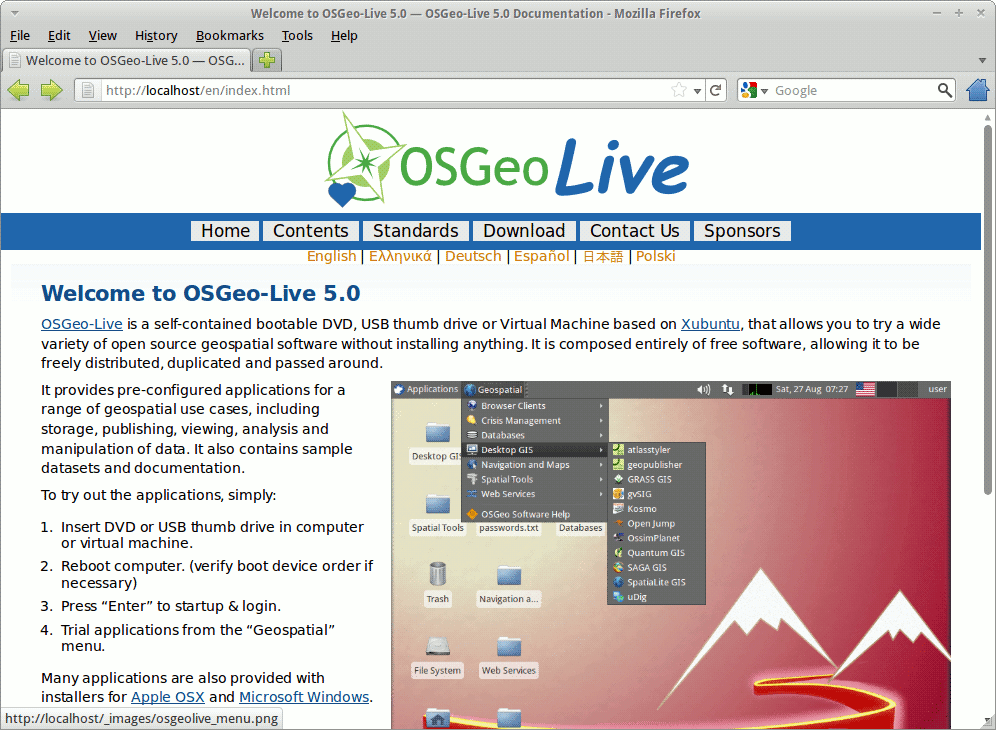
\includegraphics[width=3in]{images/00-osgeolive.png}
  \end{center}

\item Place phpinfo.php into \texttt{/usr/local/geomoose/htdocs/php}.

  This script simply calls \texttt{phpinfo()} which allows us to
  verify that Apache is processing PHP files correctly.  Also, check
  this page to make sure that the sqlite3 module is installed.  It is
  required by some of the services to keep track of features.

phpinfo.php:
\begin{verbatim}
<?php
phpinfo();
?>
\end{verbatim}

\item Test PHP: \url{http://localhost/geomoose/php/phpinfo.php}

  You should see a result similar to:
  \begin{center}
    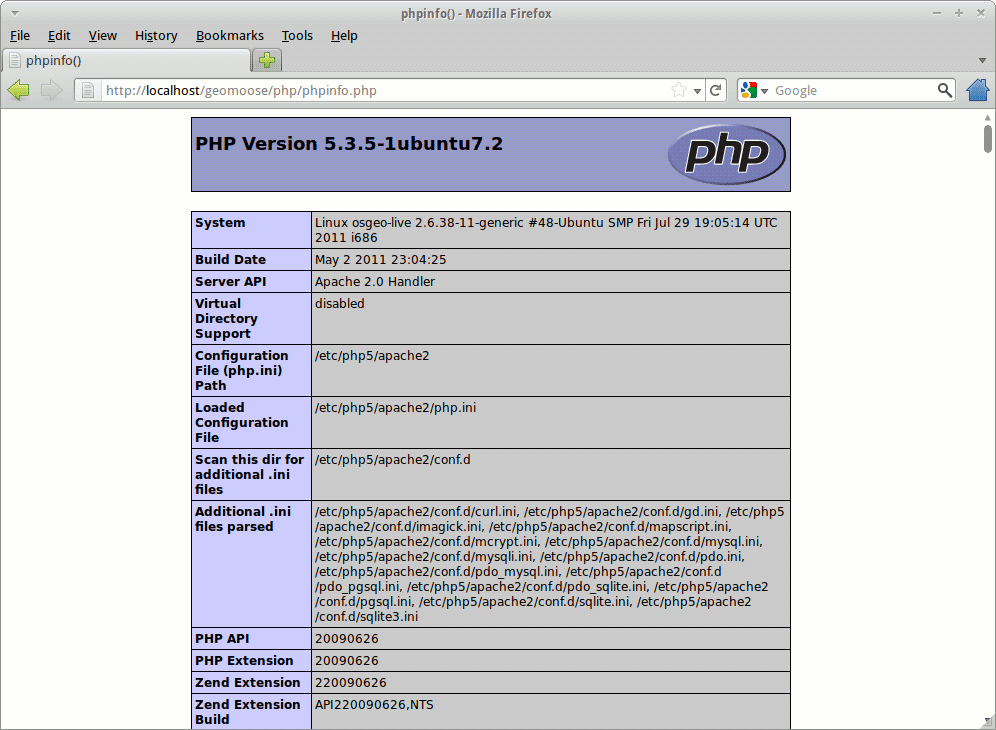
\includegraphics[width=3in]{images/00-php.png}
  \end{center}

\item Test GeoMOOSE: \url{http://localhost/geomoose/geomoose.html}

  You should see GeoMOOSE load and display the initial map.
  \begin{center}
    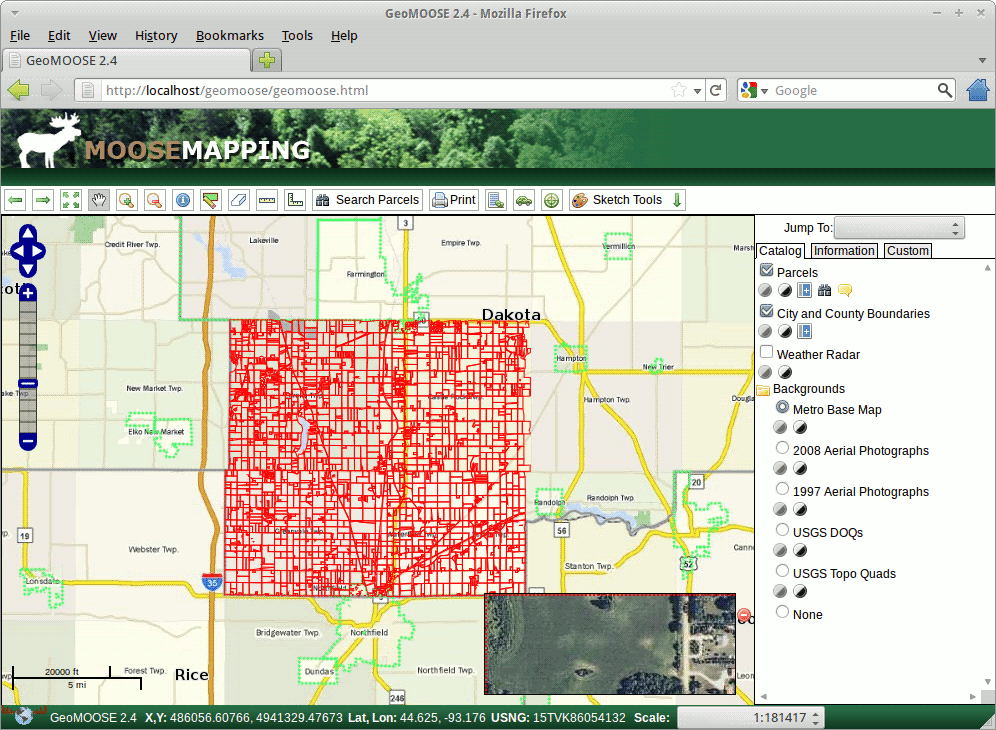
\includegraphics[width=3in]{images/00-geomoose.png}
  \end{center}
\end{enumerate}

\section*{Exercise 1: Exploring the interface}
\subsection*{Basic Tools}
Note the tools in the toolbar above the map.  If you hover over the
tool you will see the tool's name.  Try the various tools.  There are
two types of tools in GeoMOOSE.  Some tools like ``pan'' and ``zoom''
stay active after they are selected.  Other tools such as ``Print''
perform an immediate action and whatever tool was selected before
remains active.
 
\subsection*{Other Tools/Services}
Tools are also separated by if they are implemented in the client in
JavaScript, or if they are implemented by querying the server.  The
tools that query the server are known as services.

\subsection*{Catalog}
This is where the layers reside.  Notice there are also tools
available under each layer that apply to that particular layer.

\subsection*{Final Notes}
All of the tools, services, and layers are configured in the
Mapbook.  We will explore the Mapbook later.

\section*{Exercise 2: Creating a new GeoMOOSE instance}
So far we have been working with the demonstration install on the
LiveDVD.  For the purposes of the workshop, we will make a new
installation so we can make changes without disturbing the demo. To do
this, first copy the existing demo install to a new folder.  Then,
configure the new folder to update the paths stored in the
configuration files. Finally, create a symlink so Apache can see the
files in the htdocs directory.

\begin{alltt}
user@osgeo-live:/usr/local\$ \textbf{sudo cp -r geomoose geomoose-class}
user@osgeo-live:/usr/local\$ \textbf{sudo chown -R user geomoose-class}
user@osgeo-live:/usr/local\$ \textbf{cd geomoose-class}
user@osgeo-live:/usr/local/geomoose-class\$ \textbf{./configure --with-url-path=/geomoose-class} \verb'\'
\textbf{                                              --with-temp-directory=/tmp/} \verb'\'
\textbf{                                              --with-mapfile-root=/usr/local/geomoose-class/maps/}
configure: creating ./config.status
config.status: creating Makefile
config.status: creating ms4w/Apache/htdocs/geomoose2.pkg.html
config.status: creating conf/mapbook.xml
config.status: creating conf/mapbook_webmercator.xml
config.status: creating conf/settings.ini
config.status: creating geomoose2_httpd.conf
config.status: creating maps/temp_directory.map
user@osgeo-live:/usr/local/geomoose-class\$ \textbf{sudo ln -s /usr/local/geomoose-class/htdocs} \verb'\'
\textbf{                                                       /var/www/geomoose-class}
user@osgeo-live:/usr/local/geomoose-class\$ 
\end{alltt}

\noindent
You should now be able to view the ``new'' interface at \url{http://localhost/geomoose-class/geomoose.html}.
\begin{center}
  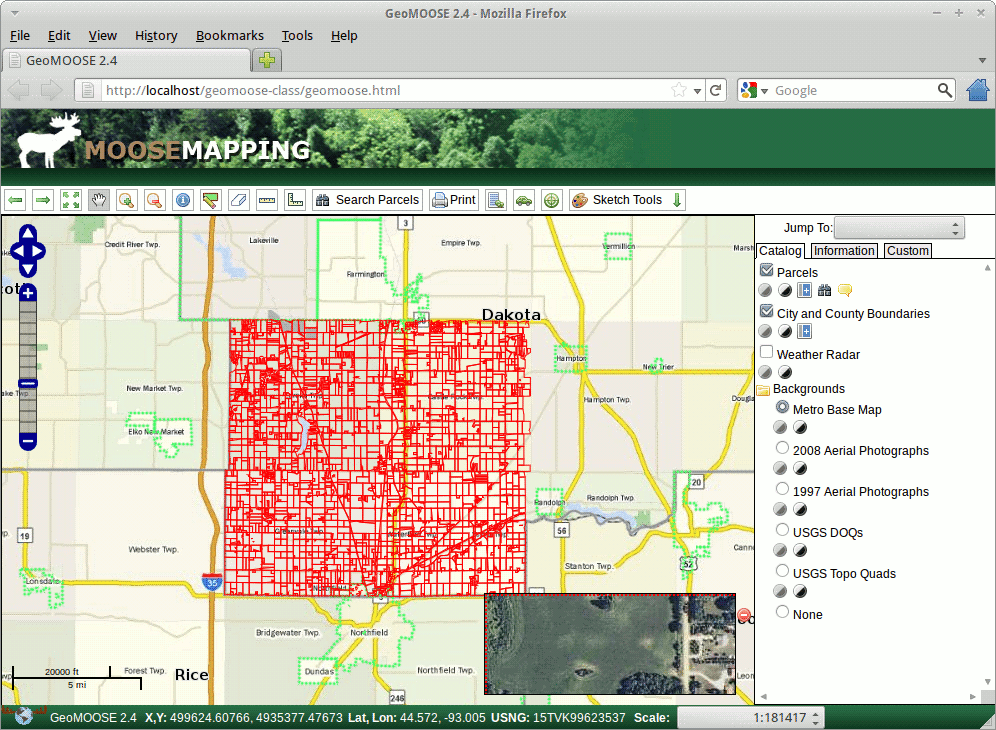
\includegraphics[width=3in]{images/02-results.png}
\end{center}

\section*{Exercise 3: Customizing the interface}
In this exercise we will customize the new interface.  We will start
by changing the title and skin.  This is done in the
\texttt{geomoose.html} file.

\begin{enumerate}
\item Open the \texttt{geomoose.html} file in the \texttt{htdocs}
  folder of the new geomoose-class instance in a text editor.
\item Navigate to the \verb|<title>GeoMOOSE 2.4</title>| line and
  change it to read \\ \verb|<title>GeoMOOSE 2.4 - Workshop</title>|.
\item Now navigate to around line 45 where the skins are defined.
  Comment out the green skin and uncomment the blue skin.  If you are
  familiar with CSS, take a look at the skin's CSS file.
\item Reload the geomoose-class page in the browser to see the changes
\end{enumerate}

\begin{center}
  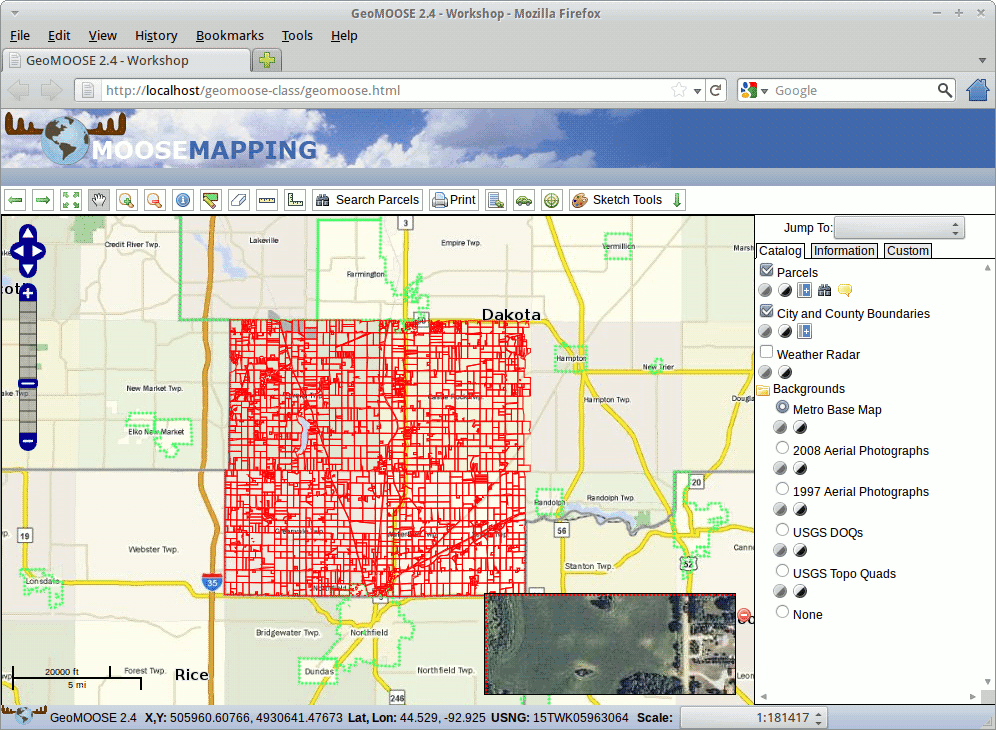
\includegraphics[width=3in]{images/03-results.png}
\end{center}

\section*{Exercise 4: Customizing the map}
In this exercise we will customize the map display.  To work with the
layers we will be adding later, we need to change the project from
EPSG:26915 (UTM 15) to EPSG:900913 (Web Mercator).  We will also need
to change the extents of the map to be the world, and allow the user
to zoom out farther.

\begin{description}
\item[Changing the projection:] The projection needs to be changed in
  two places.  First in the \texttt{settings.ini} file in the
  \texttt{conf} directory.  This file controls the PHP services.  Open
  the settings.ini file in a text editor and change the line that
  reads \verb|projection=EPSG:26915| to read
  \verb|projection=EPSG:900913| and save the file.

  Next, open the \texttt{mapbook.xml} file in a text editor. Find the
  line that sets the projection.  Change the projection from
  \verb|EPSG:26915| to \verb|EPSG:900913|.  It should look like
  \begin{verbatim}
		<param name="projection">EPSG:900913</param>
  \end{verbatim}
  when you are done.
  
\item[Changing the extents:] Continuing in the mapbook, find the lines
  that configure the \verb|max_extent| and \verb|initial_extent|.
  Change both extents to \verb|-20037508.34,-20037508.34,20037508.34,20037508.34|.  It should look like
  \begin{verbatim}
		<param name="max_extent">-20037508.34,-20037508.34,20037508.34,20037508.34</param>
		<param name="initial_extent">-20037508.34,-20037508.34,20037508.34,20037508.34</param>
  \end{verbatim}
  when you are done.

\item[Changing the Jump To list:] Continuing in the mapbook, find the
  lines that define the Jump To list. Change it to include entries for
  the world and New York City.

\begin{verbatim}
		<param name="zoomto['Jump To:']"><![CDATA[
		{
			'World' : [-20037508.34,-20037508.34,20037508.34,20037508.34],
			'New York City' : [-8242894,4965204,-8227290,4994963]
		}
\end{verbatim}

\item[Adding to the available scales:] Find the scales configuration parameter and change it to read

\begin{verbatim}

\end{verbatim}

\item[Wrap up:] Look at the other parameters available in the
  \verb|<configuration/>| section of the mapbook.

\item[Test it:] Reload the geomoose-class page.
\end{description}

\begin{center}
  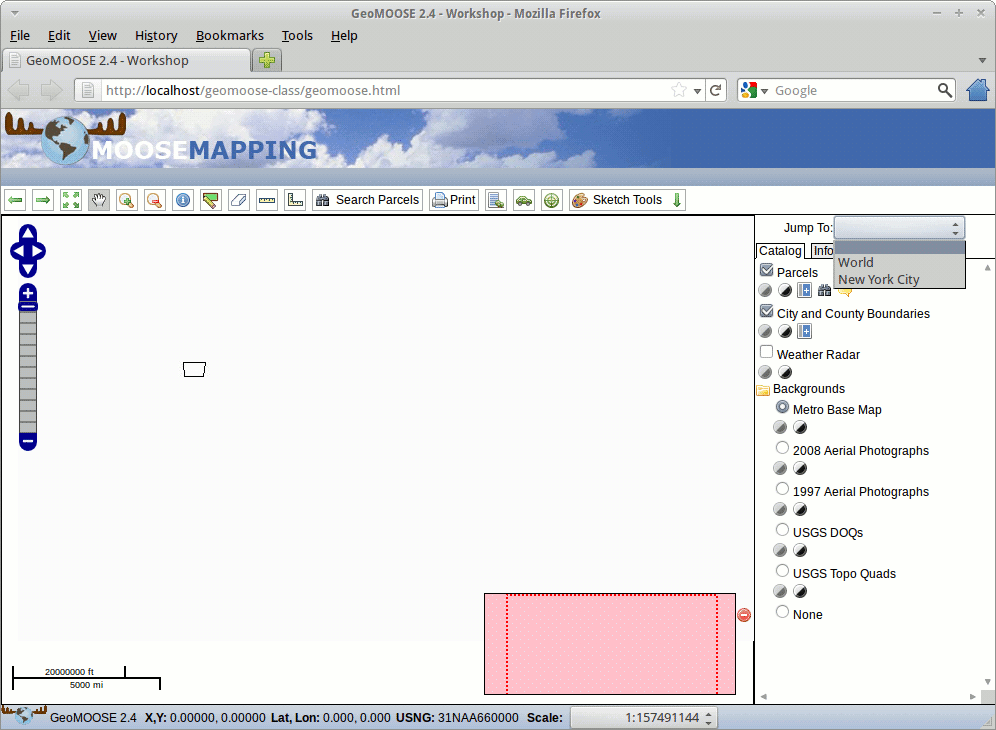
\includegraphics[width=3in]{images/04-results.png}
\end{center}

\section*{Exercise 5: Adding a WMS layer}
There are to parts to adding a layer to GeoMOOSE.  First a
\verb|<map-source/>| must be defined to tell GeoMOOSE how to access
the data.  Then a \verb|<layer/>| entry must be added to the catalog.
This is split because the layer can be included in the catalog
multiple times.

\begin{description}
\item[Adding the map-source:] Under the definition for the highlight
  layer add the following to define the new map-source.

\begin{verbatim}
	<map-source name="geoserver" type="wms">
		<url>http://localhost:8082/geoserver/ows?</url>
		<layer name="tiger-ny"/>
		<param name="TRANSPARENT" value="true"/>
	</map-source>
\end{verbatim}

\item[Adding the layer:] Locate the \verb|<catalog/>| section.  Add
  the following to add the layer to the catalog.
\begin{verbatim}
		<layer title="Tiger-NY" src="geoserver/tiger-ny" status="on"/>
\end{verbatim}

\item[Test it:] Reload the geomoose-class page.
\end{description}

\begin{center}
  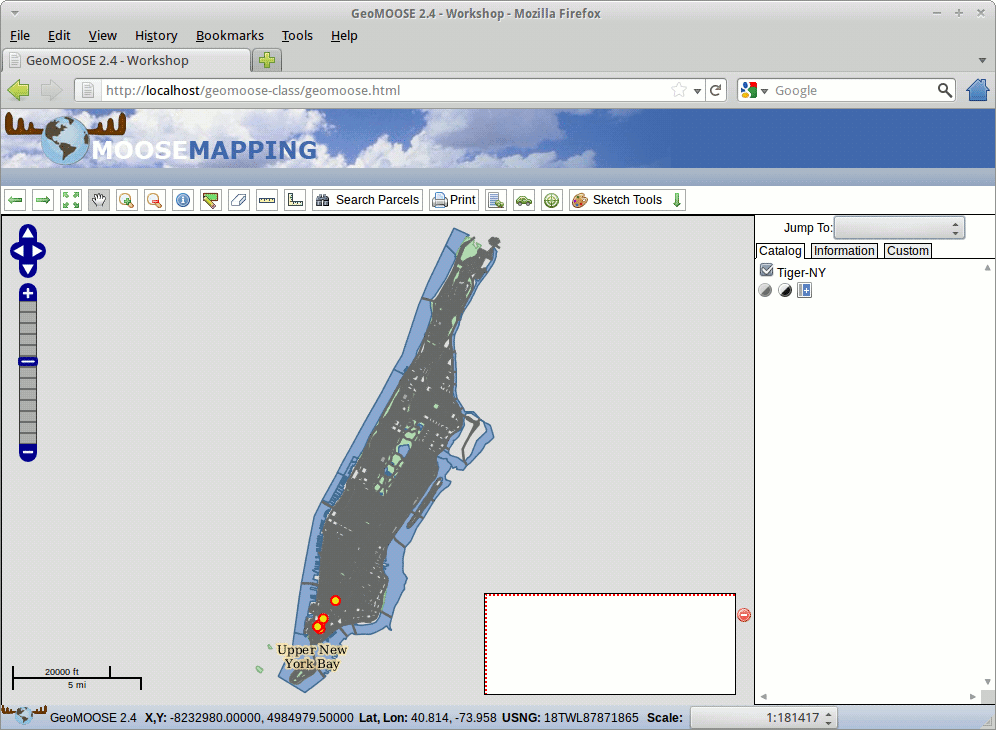
\includegraphics[width=3in]{images/05-results.png}
\end{center}

\section*{Exercise 6: Adding a MapServer Layer}
Adding a MapServer layer is similar to adding a WMS layer.  This has
been the traditional way to add a layer to GeoMOOSE and still is more
flexible than the WMS route.  The main advantages with the MapServer
route right now are that it gives you more control over the
presentation (even if you are just laundering a WMS layer) and the
standard services currently work better with MapServer layers. We are
working on improving the WMS functionality for GeoMOOSE 2.6.

This exercise will add the countries layer from the Natural Earth
dataset that is included on the LiveDVD.  We will need to create a
Mapfile to tell MapServer how to render the layer.  Then we will add
that layer to the catalog.  Finally, we will intentionally break the
layer to demonstrate how to troubleshoot typical problems.

\begin{description}
\item[Creating the Mapfile]: We will reuse some of the architecture
  from the demo layers.  
  \begin{enumerate}
    \item Under \verb|/usr/local/geomoose-class/maps|
      create a directory called \verb|natural_earth| and in
      \verb|natural_earth| create a directory called \verb|countries|.
    \item Copy the MapServer Mapfile (\verb|natural_earth.map|) into
      the \verb|countries| directory.  If you are familiar with
      MapServer, this is just a standard Mapfile.  If you are not
      familiar with MapServer, this is just a text file.

\begin{figure*}

\caption{natural\_earth.map}

\tiny
      \begin{verbatim}
MAP
	NAME 'natural_earth'
	SIZE 800 650
	STATUS ON
	EXTENT -20037508.34 -20037508.34 20037508.34 20037508.34
        UNITS METERS

	INCLUDE "../../geomoose_globals.map"

	WEB
		METADATA
			'ows_title' 'Countries'
			'ows_srs' 'EPSG:26915 EPSG:4326 EPSG:900913'
		END
	END

	PROJECTION
		'init=epsg:900913'
	END

	LEGEND
	      STATUS ON
	      LABEL
		TYPE TRUETYPE
		FONT vera_sans
		SIZE 8
		COLOR 0 0 0
	      END		
	END	

	LAYER
	    NAME 'countries'
	    DATA '/home/user/data/natural_earth/10m_admin_0_countries'
	    STATUS ON
	    TYPE LINE
	    MINSCALE 1000
	    SYMBOLSCALE 200000
	    PROJECTION
 		"init=epsg:4326"
	    END
	    LABELITEM 'NAME'
	      CLASS
		 NAME "Country Boundary"
		 STYLE
		   SYMBOL 'circle'
		   SIZE 3
		   MINSIZE 3
		   MAXSIZE 5
		   COLOR 210 210 210
		 END
		 STYLE
		   SIZE 1
		   MINSIZE 1
		   MAXSIZE 3
		   # WIDTH 1
		   COLOR 50 50 50
		 END
	        LABEL
		  TYPE TRUETYPE
		  FONT vera_sans-bold
		  FORCE TRUE
		  MINSIZE 8
		  SIZE 10
		  MAXSIZE 12
		  COLOR 0 0 0
		  OUTLINECOLOR 232 232 232
		  BUFFER 4
	        END
	      END
	END 
END ## end Map
      \end{verbatim}
\end{figure*}

  \end{enumerate}
\item[Adding the layer to the Mapbook:] This is similar to adding the
  WMS layer.
  \begin{enumerate}
    \item Open the mapbook in a text editor (\verb|/usr/local/geomoose-class/conf/mapbook.xml|)
    \item Add the natural-earth map-service above the \verb|geoserver|
      service.  Note: the order of the map-services controls the
      default draw order of the layers.
      \begin{verbatim}
	<map-source name="natural_earth" type="mapserver" queryable="true">
		<file>./workshop/natural_earth/natural_earth.map</file>
		<layer name="countries"/>
		<param name="TRANSPARENT" value="true"/>
	</map-source>
      \end{verbatim}
    \item Add the layer to the catalog... maybe under the Tiger-NY
      layer, but really anywhere you want.
      \begin{verbatim}
		<layer title="Countries" src="natural_earth/countries" status="on"/>
      \end{verbatim}
  \end{enumerate}
\end{description}

\begin{center}
  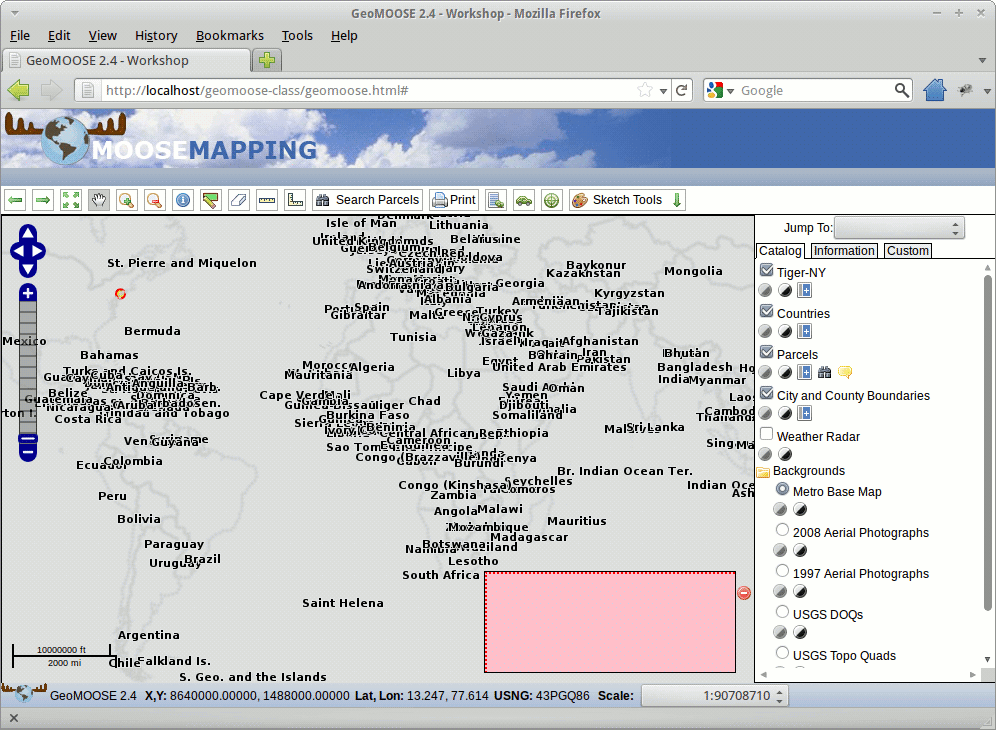
\includegraphics[width=3in]{images/06-results.png}
\end{center}

\subsection*{Breaking it:}
\begin{description}
\item[Break the Mapfile:] Edit the \verb'natural_earth.map' file
  and introduce an error somewhere.  For example change
  \verb'LAYER' to \verb'LLAYER'.  Reload the layer in the
  interface and see what it does.  Look in Firebug and look for
  the link to the natural earth layer.  Open that link in a new
  tab to see the error message from MapServer.
\item[Break the Mapbook:] \hfill \\
  \begin{enumerate}
  \item Introduce an error into the mapbook. Change
    \verb|<?xml version="1.0"?>| into
    \verb|<?xxml version="1.0"?>|.  Reload the interface and see
    what it does.
  \item Restore the mapbook and reload the interface to make
    sure it works again.
  \item Introduce a different error the mapbook.  Change the
    name for the \verb|natural_earth| map-source so it doesn't match
    the path for that layer in the catalog.  I.E. change

    \verb|<map-source name="natural_earth" type="mapserver" queryable="true">|

    to

    \verb|<map-source name="natural_earth_" type="mapserver" queryable="true">|
  \item Reload the interface and see what it does.
  \end{enumerate}
\end{description}

\section*{Exercise 7: Custom Extensions}
  See \url{http://www.geomoose.org/developer/extensions.html}.
\section*{Exercise 8: Custom Services}
  See \url{http://www.geomoose.org/developer/services.html}.

\end{document}
